\documentclass[12pt,a4paper]{article}

% -----------------------------
% Packages
% -----------------------------
\usepackage[utf8]{inputenc}
\usepackage[T1]{fontenc}
\usepackage{lmodern}
\usepackage{geometry}
\usepackage{setspace}
\usepackage{graphicx}
\usepackage{float}
\usepackage{booktabs}
\usepackage{array}
\usepackage{hyperref}
\usepackage{caption}
\usepackage{amsmath}
\usepackage{enumitem}

% -----------------------------
% Page setup
% -----------------------------
\geometry{
	a4paper,
	left=2.5cm,
	right=2.5cm,
	top=2.5cm,
	bottom=2.5cm
}

\setstretch{1.15}

\hypersetup{
	colorlinks=true,
	linkcolor=black,
	citecolor=black,
	urlcolor=blue
}

% -----------------------------
% Document information
% -----------------------------
\newcommand{\projecttitle}{EEG-Based Mental Stress Detection}
\newcommand{\coursename}{Data Science Capstone Project}
\newcommand{\submissiondate}{25 June 2026}
\newcommand{\authors}{Yoana Agafonova and Iliana Hristova}

\begin{document}
	
	% =====================================================
	% TITLE PAGE
	% =====================================================
	\begin{titlepage}
		\centering
		
		{\Large \coursename \par}
		
		\vspace{2cm}
		
		{\Huge \textbf{\projecttitle} \par}
		
		\vspace{1.5cm}
		
		{\Large Final Report \par}
		
		\vspace{2cm}
		
		\begin{tabular}{ll}
			\textbf{Course:} & \coursename \\
			\textbf{Authors:} & \authors \\
			\textbf{Submission Date:} & \submissiondate \\
		\end{tabular}
		
		\vfill
		
		{\large IMC University of Applied Sciences Krems \par}
		
	\end{titlepage}
	
	\pagenumbering{roman}
	
	% =====================================================
	% ABSTRACT
	% =====================================================
	\begin{abstract}
		This report presents a data science project for EEG-based mental stress detection. The aim of the project is to classify EEG recordings into stress and non-stress states using machine learning. The dataset consists of EEG recordings collected under several experimental conditions, including complex mathematical problem solving, Trier mental challenge testing, Stroop colour word testing, horror video stimulation, and relaxing music listening. The stress-inducing conditions were grouped into the stress class, while the relaxing music condition was used as the non-stress class.
		
		The methodology includes data loading, selection of relevant EEG channels, signal preprocessing, window-based segmentation, feature extraction, and model evaluation. Five EEG channels were used: AF3, T7, Pz, T8, and AF4. The EEG signals were filtered using a 0.5--45 Hz bandpass filter and divided into 10-second windows. For each window, statistical features and frequency-band power features were extracted. Several machine learning models were compared, including Logistic Regression, Random Forest, Support Vector Machine, K-Nearest Neighbors, and Gradient Boosting.
		
		The results show that window-based classification improves the amount of available training data, but evaluation must be performed carefully because windows from the same recording can be highly similar. Therefore, GroupKFold validation was used to keep windows from the same EDF recording together. Under this stricter evaluation, Gradient Boosting achieved the best Macro F1-score. The final model performed well in detecting stress windows, but struggled with the minority non-stress class, mainly due to class imbalance. Overall, the project demonstrates that EEG features can be used for stress detection, while also highlighting the challenges of imbalanced biomedical signal classification.
	\end{abstract}
	
	\newpage
	\tableofcontents
	\newpage
	
	\pagenumbering{arabic}
	
	% =====================================================
	% 1. INTRODUCTION
	% =====================================================
	\section{Introduction}
	
	\subsection{Problem Statement}
	
	Mental stress is an important factor affecting health, cognitive performance, productivity, and general well-being. In many situations, stress is assessed through questionnaires or self-reports. Although these methods are easy to use, they are subjective and may not always reflect the actual physiological state of a person. Because of this, physiological signals such as electroencephalography (EEG) can provide a more objective way of analyzing stress-related changes.
	
	This project focuses on building a machine learning classifier for mental stress detection using EEG recordings. The task is formulated as a binary classification problem, where EEG signal windows are classified as either stress or non-stress. The stress class includes recordings from mentally demanding or emotionally stimulating tasks, while the non-stress class includes relaxed-state recordings.
	
	\subsection{Objectives}
	
	The main objectives of this project are:
	
	\begin{itemize}
		\item to explore and understand the provided EEG dataset;
		\item to define stress and non-stress classes based on the experimental conditions;
		\item to preprocess EEG signals and select relevant EEG channels;
		\item to extract statistical and frequency-domain features from EEG windows;
		\item to train and compare several machine learning models;
		\item to evaluate the models using suitable metrics for imbalanced classification;
		\item to analyze the limitations and possible improvements of the final model.
	\end{itemize}
	
	\subsection{Dataset Overview}
	
	The dataset used in this project was provided through a soft copy link from Mendeley Data. It contains EEG recordings stored as EDF files and organized by experimental condition. The available conditions include complex mathematical problem solving, horror video stimulation, Stroop colour word testing, Trier mental challenge testing, and relaxing music listening.
	
	The selected EEG channels used in this project are AF3, T7, Pz, T8, and AF4. The recordings have a sampling frequency of 128 Hz. The four task-based conditions were grouped into the stress class, while the relaxing music condition was used as the non-stress class.
	
	\subsection{Background and Challenges}
	
	EEG data is a challenging type of biomedical signal because it can contain noise, artifacts, and strong individual variability between subjects. In addition, the dataset used in this project is imbalanced, with more stress recordings than non-stress recordings. This affects model training and evaluation because a model may achieve high accuracy by mainly predicting the majority class. For this reason, balanced accuracy and Macro F1-score are used in addition to standard accuracy.
	
	% =====================================================
	% 2. LITERATURE REVIEW
	% =====================================================
	\section{Literature Review}
	
	% We will fill this section next.
	
	% =====================================================
	% 3. METHODOLOGY
	% =====================================================
	\section{Methodology}
	
	% We will fill this section after the literature review.
	
	% =====================================================
	% 4. RESULTS
	% =====================================================
	\section{Results}
	
	\subsection{Dataset Distribution}
	
	\begin{table}[H]
		\centering
		\caption{Distribution of EEG recordings by condition.}
		\begin{tabular}{lcc}
			\toprule
			\textbf{Condition} & \textbf{Number of EDF Files} & \textbf{Class} \\
			\midrule
			Complex Mathematical Problem Solving (CMPS) & 22 & Stress \\
			Horror Video Stimulation & 22 & Stress \\
			Stroop Colour Word Test (SCWT) & 24 & Stress \\
			Trier Mental Challenge Test (TMCT) & 24 & Stress \\
			Relaxing Music & 20 & Non-stress \\
			\bottomrule
		\end{tabular}
	\end{table}
	
	\begin{table}[H]
		\centering
		\caption{Class distribution after 10-second window segmentation.}
		\begin{tabular}{lcc}
			\toprule
			\textbf{Class} & \textbf{Number of Windows} & \textbf{Percentage} \\
			\midrule
			Stress & 3037 & 86.6 \\
			Non-stress & 470 & 13.4 \\
			\bottomrule
		\end{tabular}
	\end{table}
	
	\subsection{Exploratory Data Analysis}
	
	\begin{figure}[H]
		\centering
		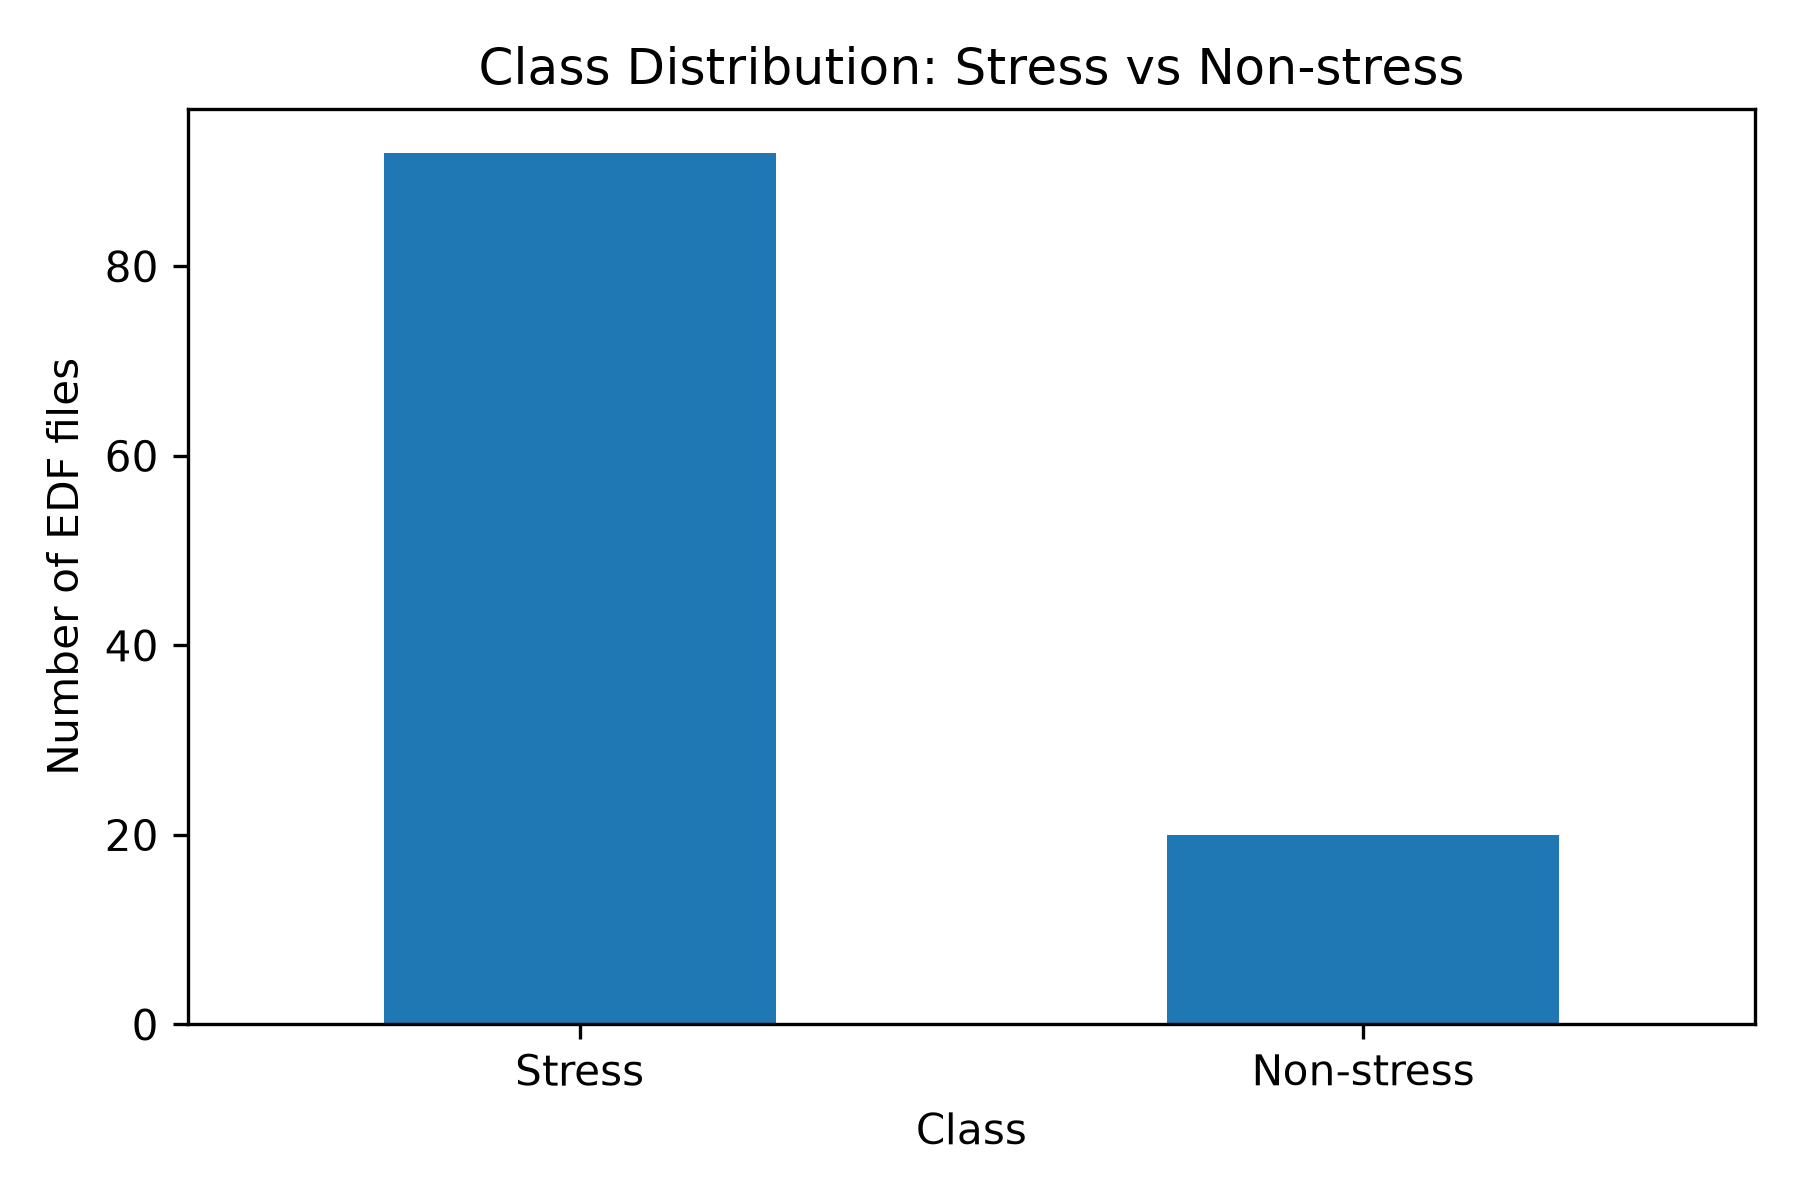
\includegraphics[width=0.75\textwidth]{../outputs/plots/class_distribution.png}
		\caption{Class distribution of stress and non-stress EEG recordings.}
		\label{fig:class_distribution}
	\end{figure}
	
	\begin{figure}[H]
		\centering
		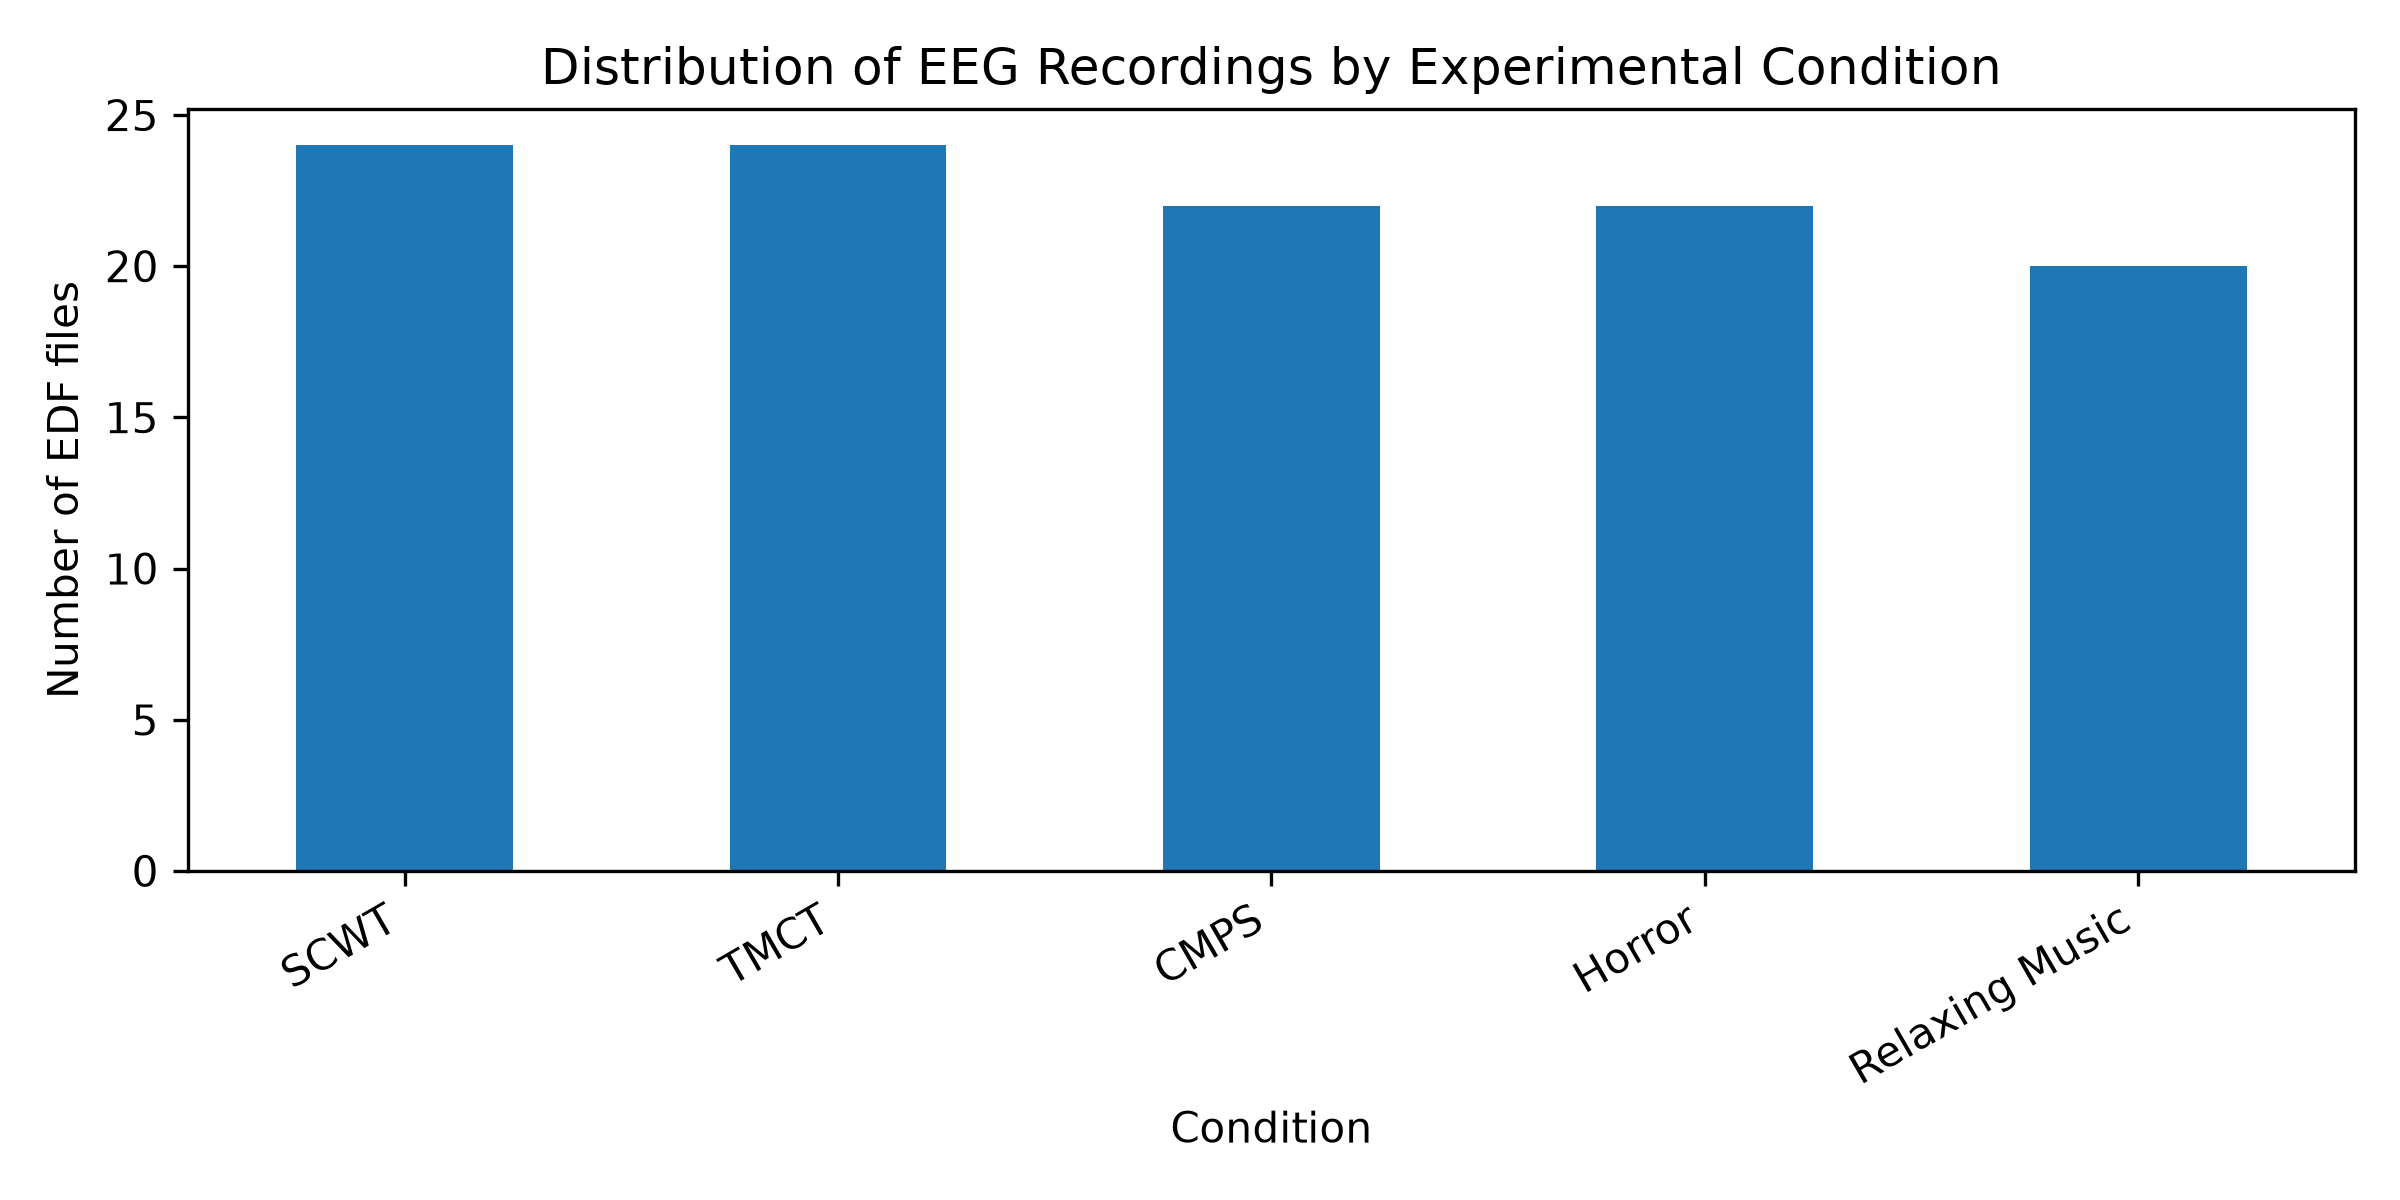
\includegraphics[width=0.85\textwidth]{../outputs/plots/condition_distribution.png}
		\caption{Distribution of EEG recordings by experimental condition.}
		\label{fig:condition_distribution}
	\end{figure}
	
	\subsection{Signal Visualization}
	
	\begin{figure}[H]
		\centering
		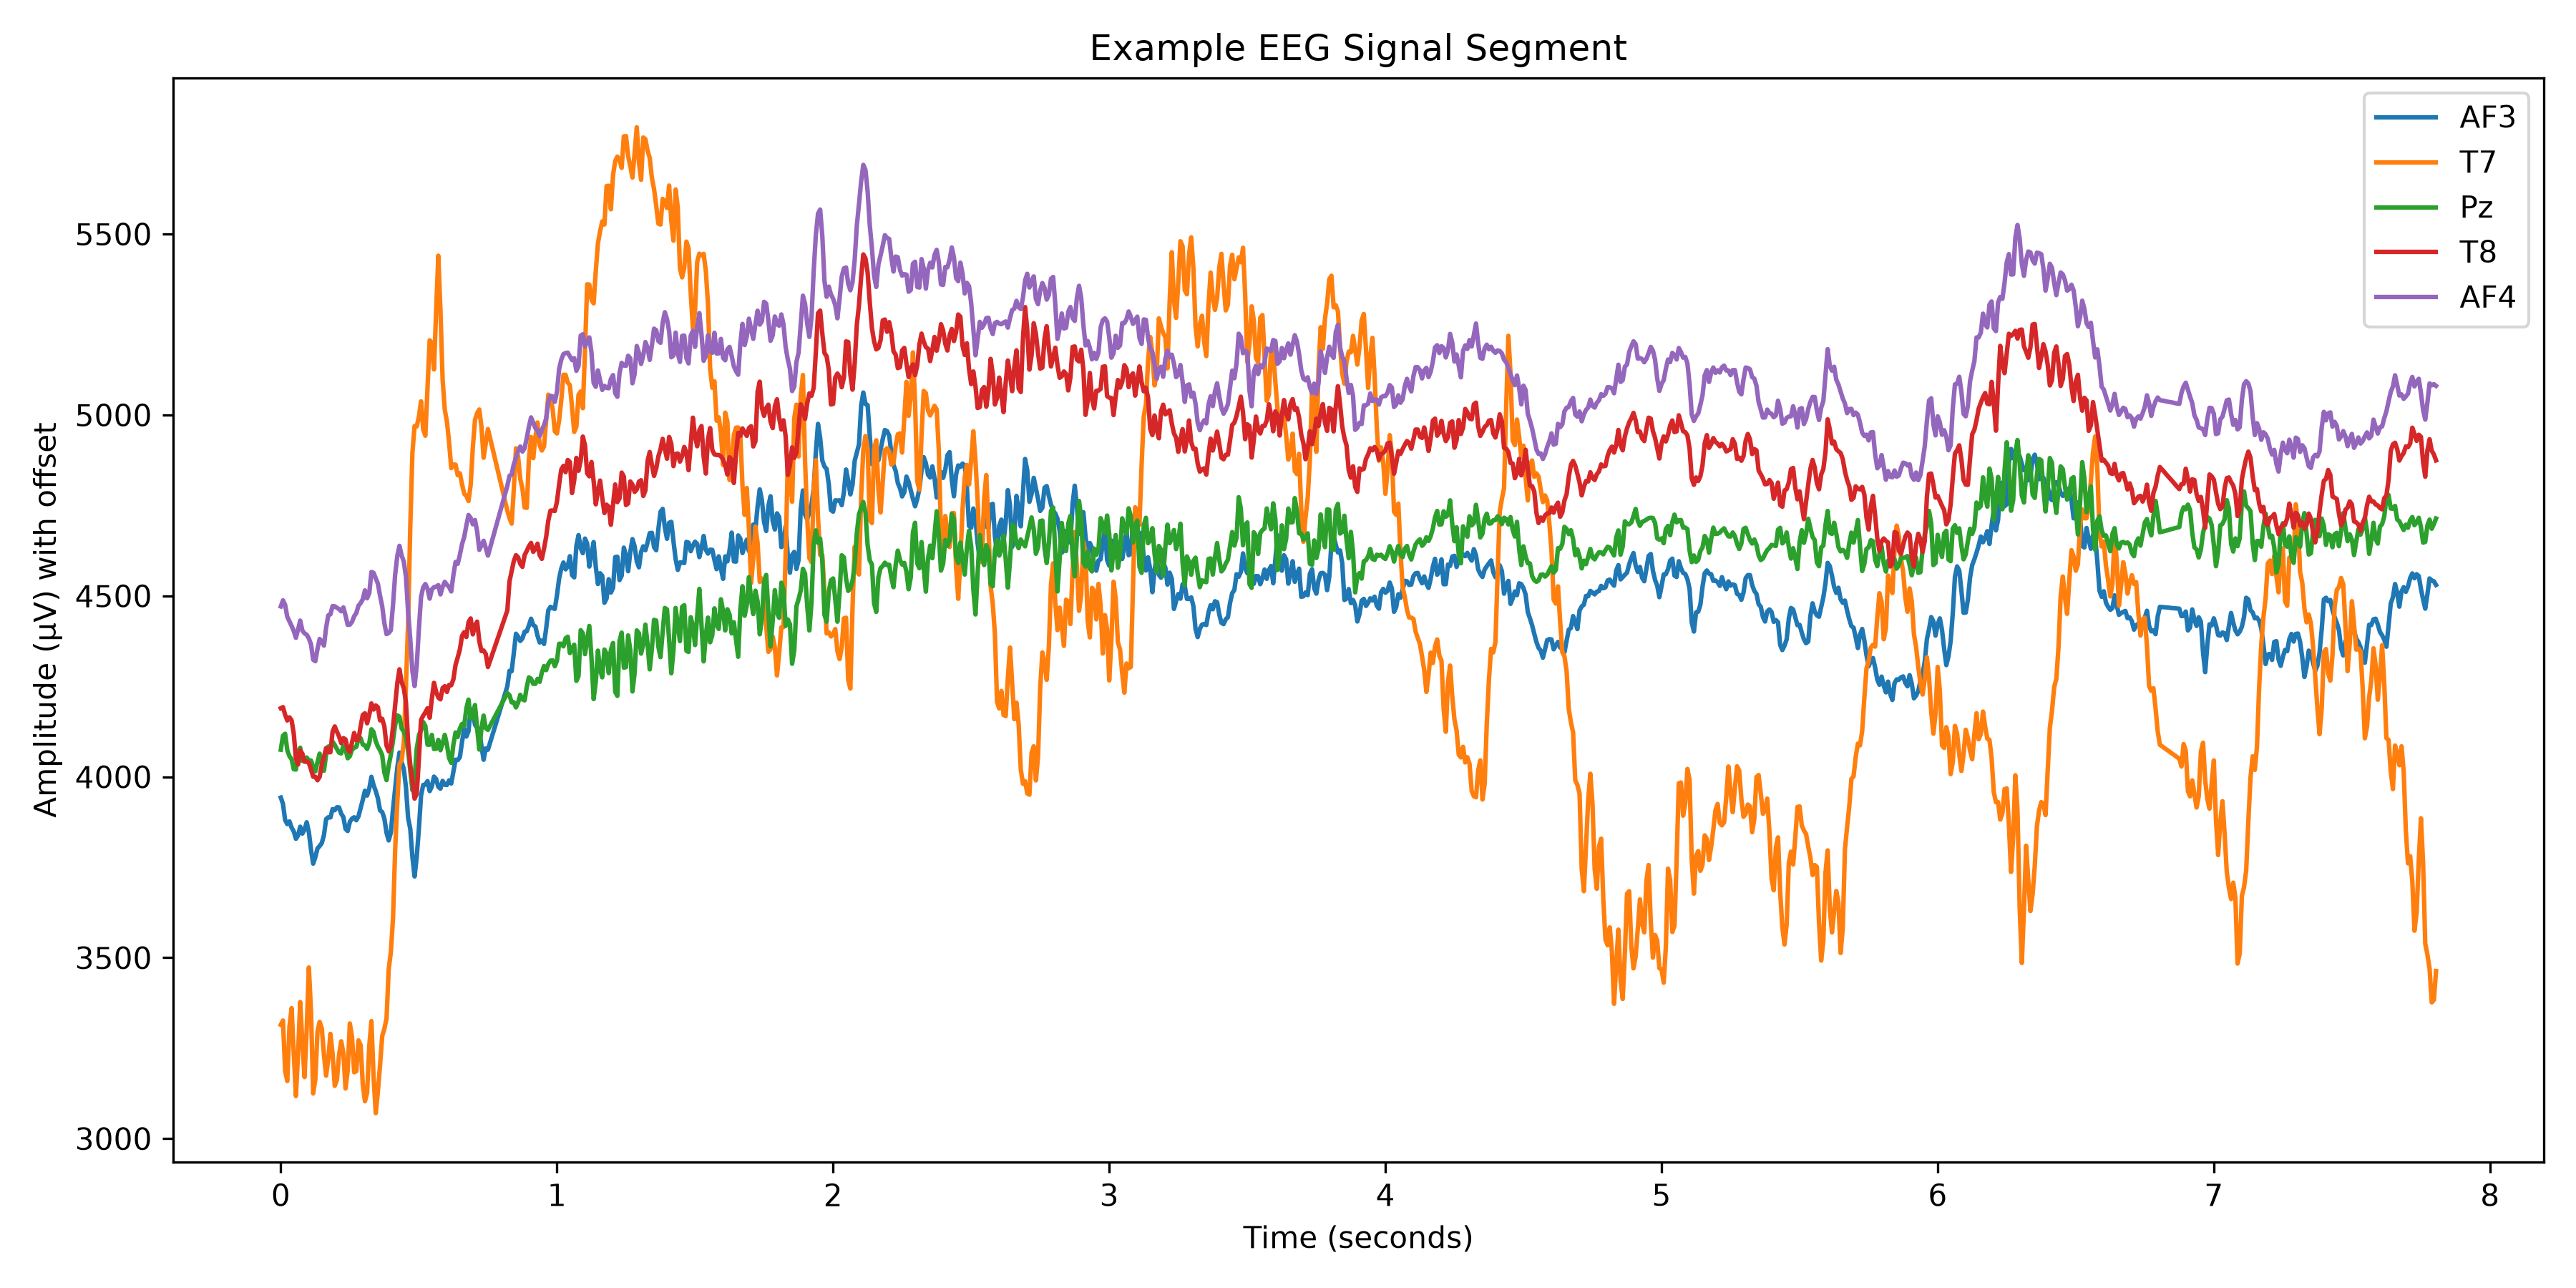
\includegraphics[width=0.9\textwidth]{../outputs/plots/example_eeg_signal.png}
		\caption{Example raw EEG signal segment from selected channels.}
		\label{fig:raw_signal}
	\end{figure}
	
	\begin{figure}[H]
		\centering
		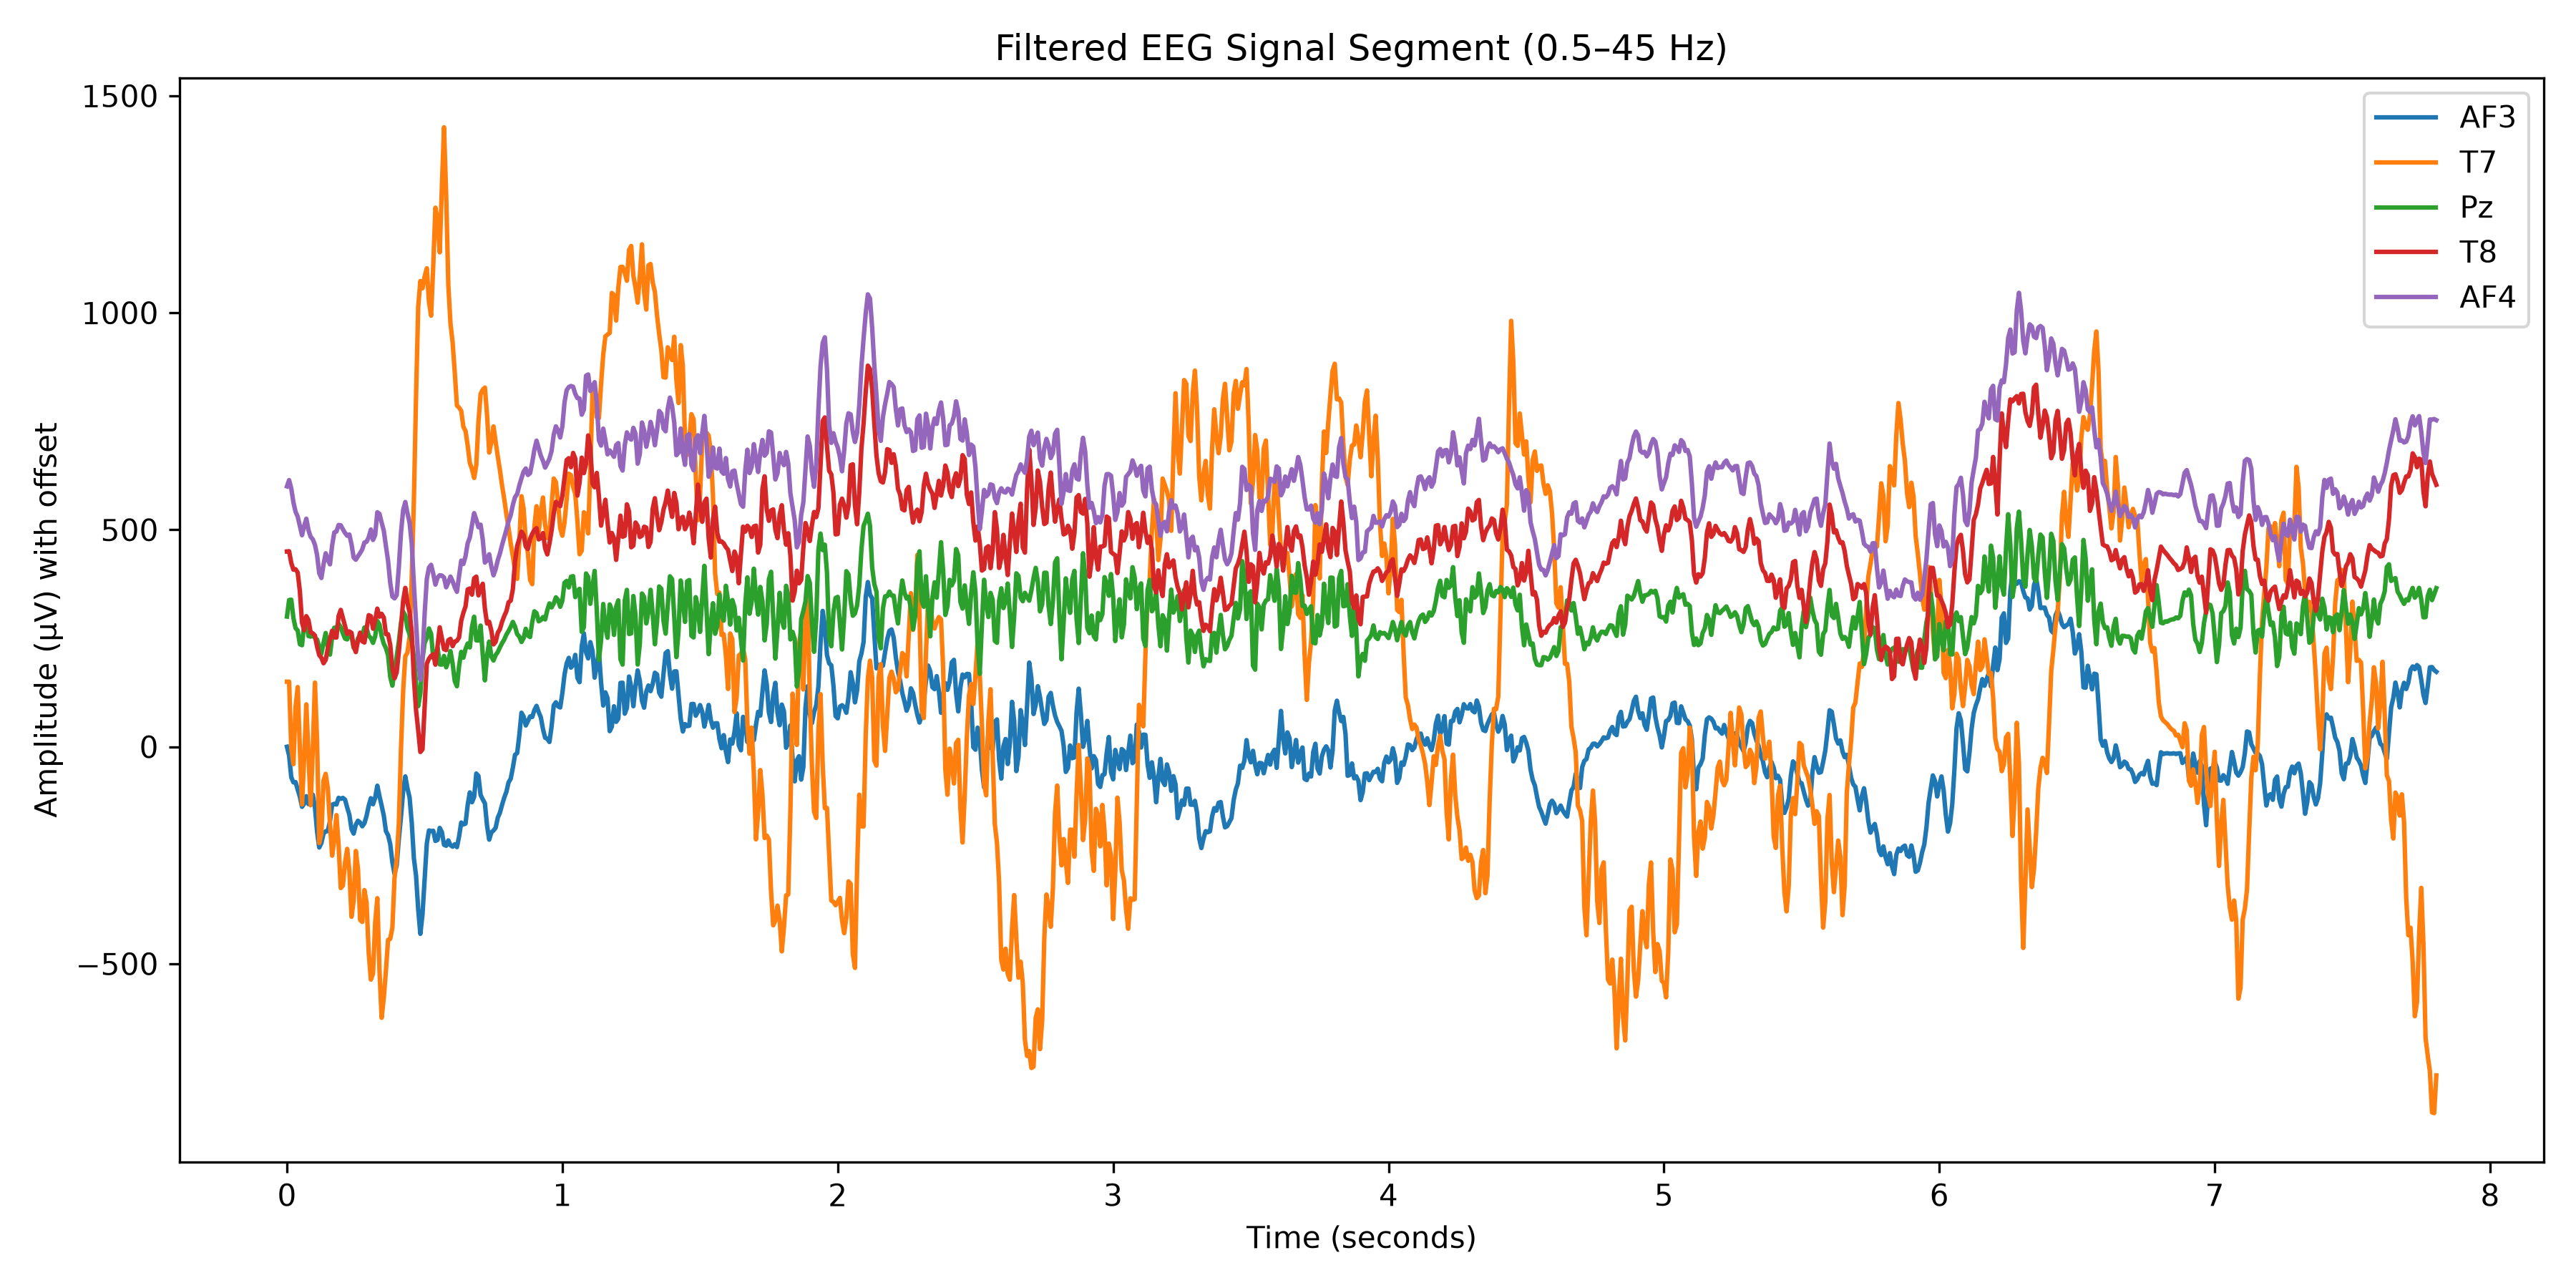
\includegraphics[width=0.9\textwidth]{../outputs/plots/filtered_eeg_signal.png}
		\caption{Filtered EEG signal segment after applying a 0.5--45 Hz bandpass filter.}
		\label{fig:filtered_signal}
	\end{figure}
	
	\subsection{Model Comparison}
	
	\begin{table}[H]
		\centering
		\caption{Model comparison using GroupKFold validation by EDF file.}
		\begin{tabular}{lccccc}
			\toprule
			\textbf{Model} & \textbf{Accuracy} & \textbf{Balanced Accuracy} & \textbf{Precision Macro} & \textbf{Recall Macro} & \textbf{F1 Macro} \\
			\midrule
			Gradient Boosting & 0.8654 & 0.5809 & 0.6758 & 0.5809 & 0.5929 \\
			KNN & 0.8349 & 0.5565 & 0.5865 & 0.5565 & 0.5625 \\
			SVM & 0.7025 & 0.6431 & 0.5685 & 0.6431 & 0.5611 \\
			Random Forest & 0.8389 & 0.5389 & 0.5884 & 0.5389 & 0.5397 \\
			Logistic Regression & 0.6541 & 0.6200 & 0.5491 & 0.6200 & 0.5224 \\
			\bottomrule
		\end{tabular}
	\end{table}
	
	\begin{figure}[H]
		\centering
		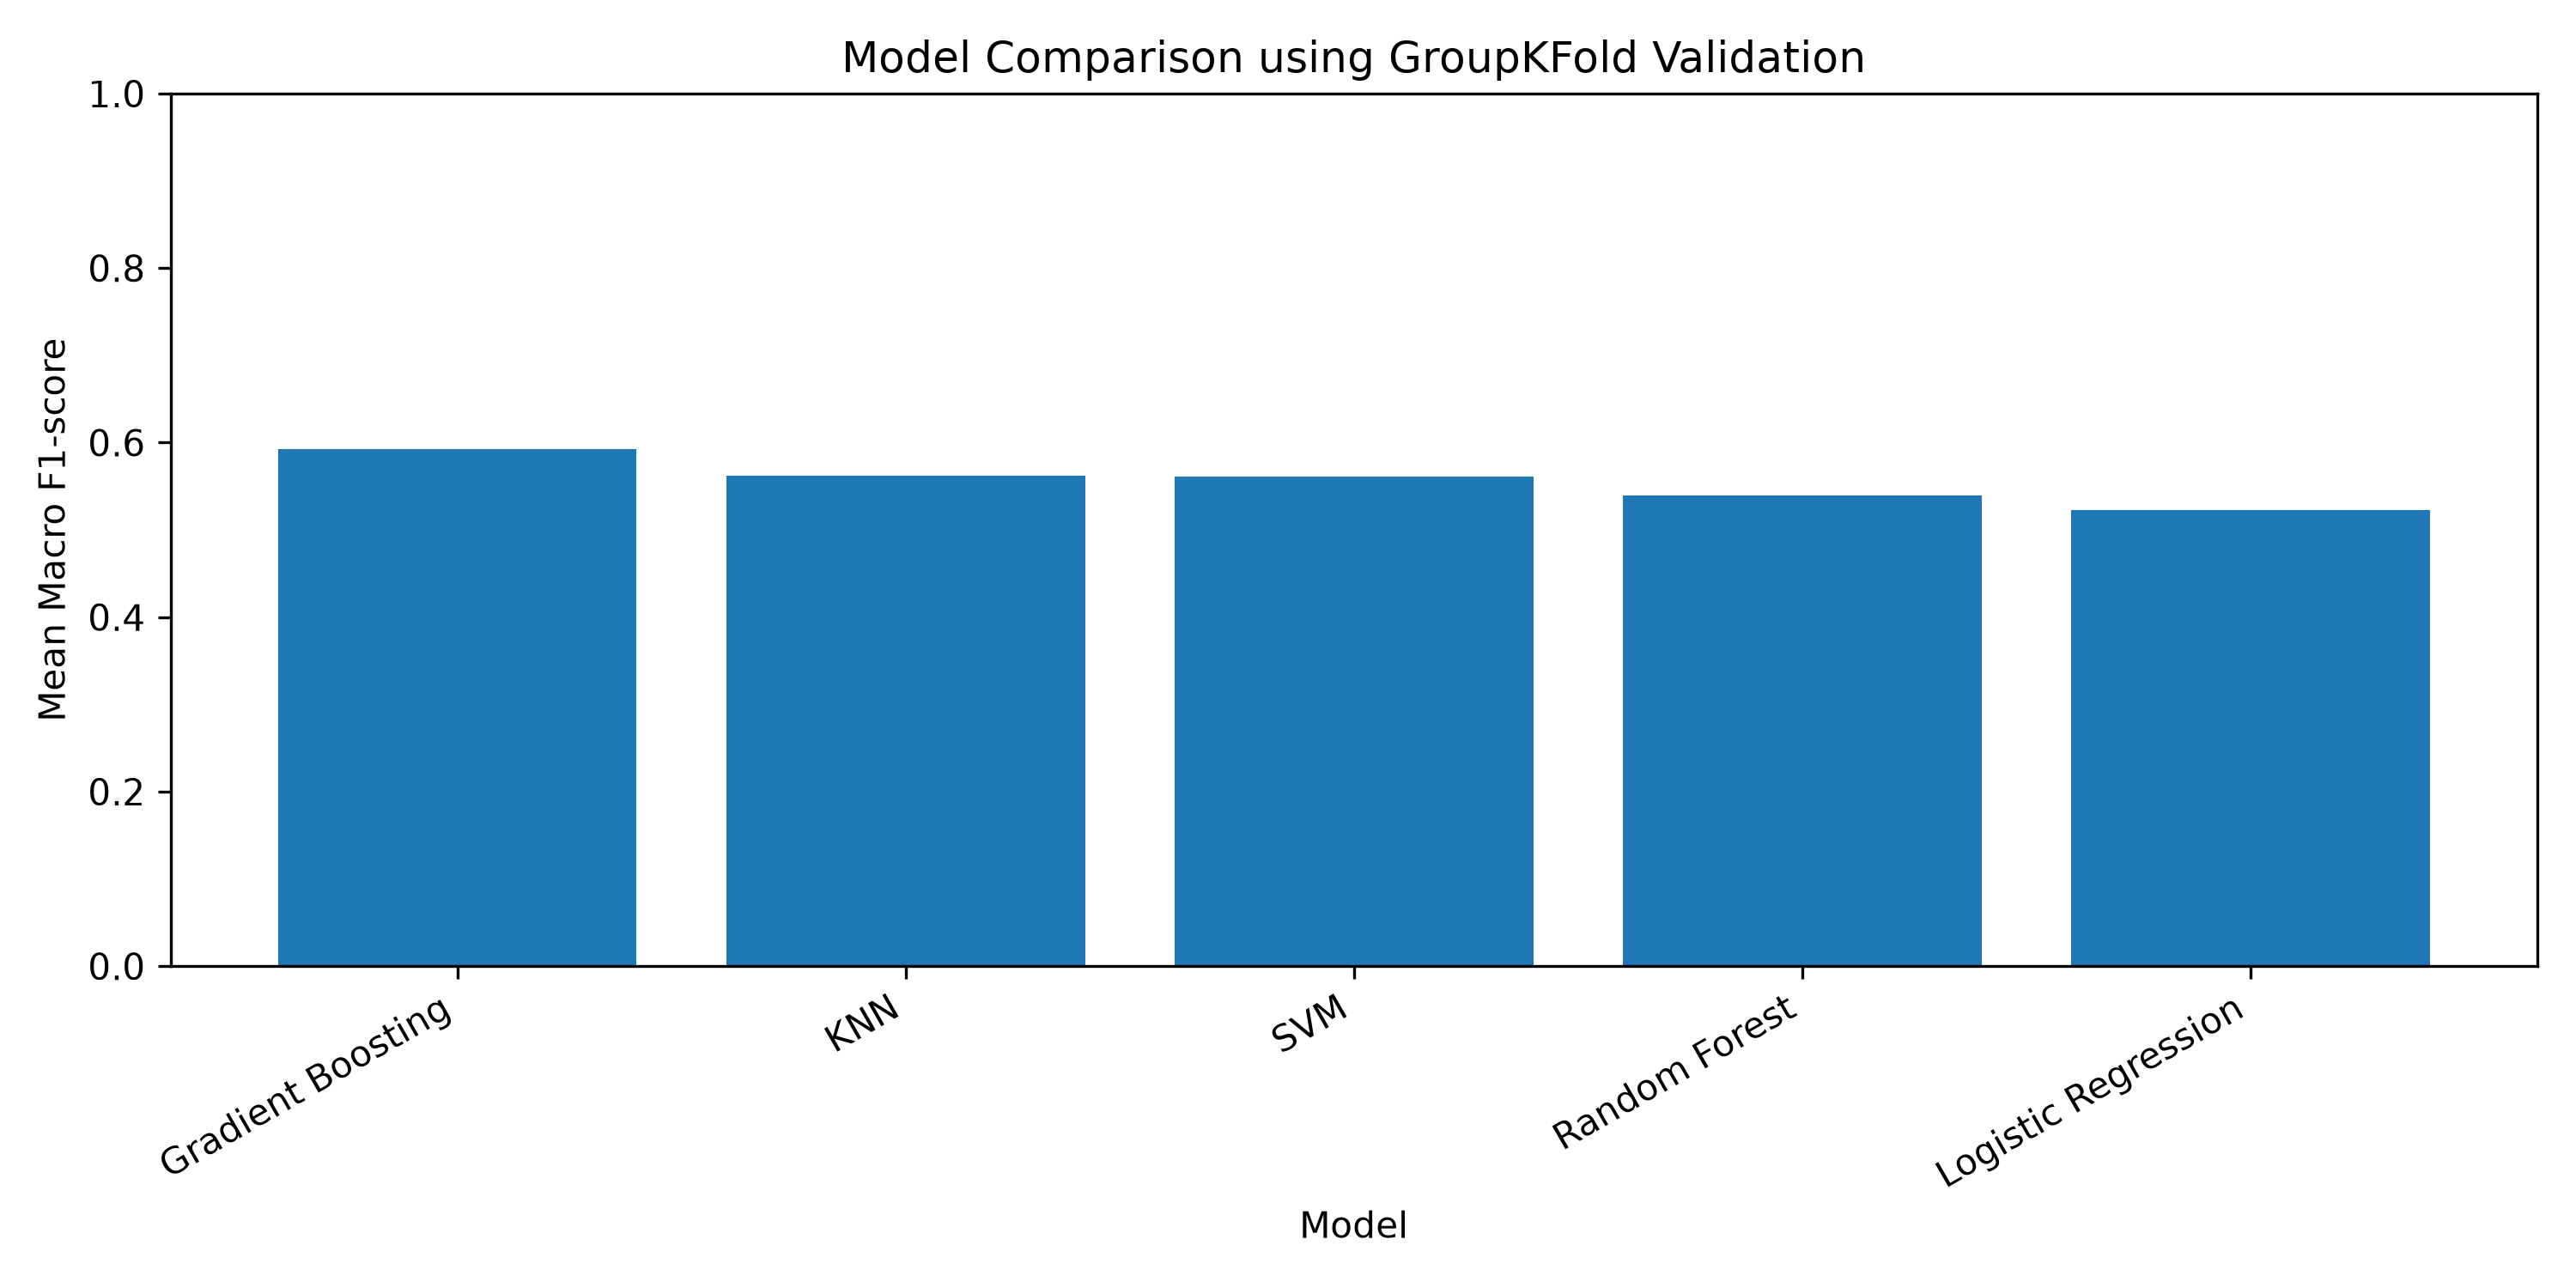
\includegraphics[width=0.85\textwidth]{../outputs/plots/model_comparison_group_cv.png}
		\caption{Model comparison using GroupKFold validation.}
		\label{fig:model_comparison_group}
	\end{figure}
	
	\subsection{Final Model Performance}
	
	\begin{table}[H]
		\centering
		\caption{Classification report for the final Gradient Boosting model.}
		\begin{tabular}{lcccc}
			\toprule
			\textbf{Class} & \textbf{Precision} & \textbf{Recall} & \textbf{F1-score} & \textbf{Support} \\
			\midrule
			Non-stress & 0.69 & 0.16 & 0.25 & 141 \\
			Stress & 0.83 & 0.98 & 0.90 & 573 \\
			\midrule
			Accuracy & -- & -- & 0.82 & 714 \\
			Macro Average & 0.76 & 0.57 & 0.58 & 714 \\
			Weighted Average & 0.80 & 0.82 & 0.77 & 714 \\
			\bottomrule
		\end{tabular}
	\end{table}
	
	\begin{figure}[H]
		\centering
		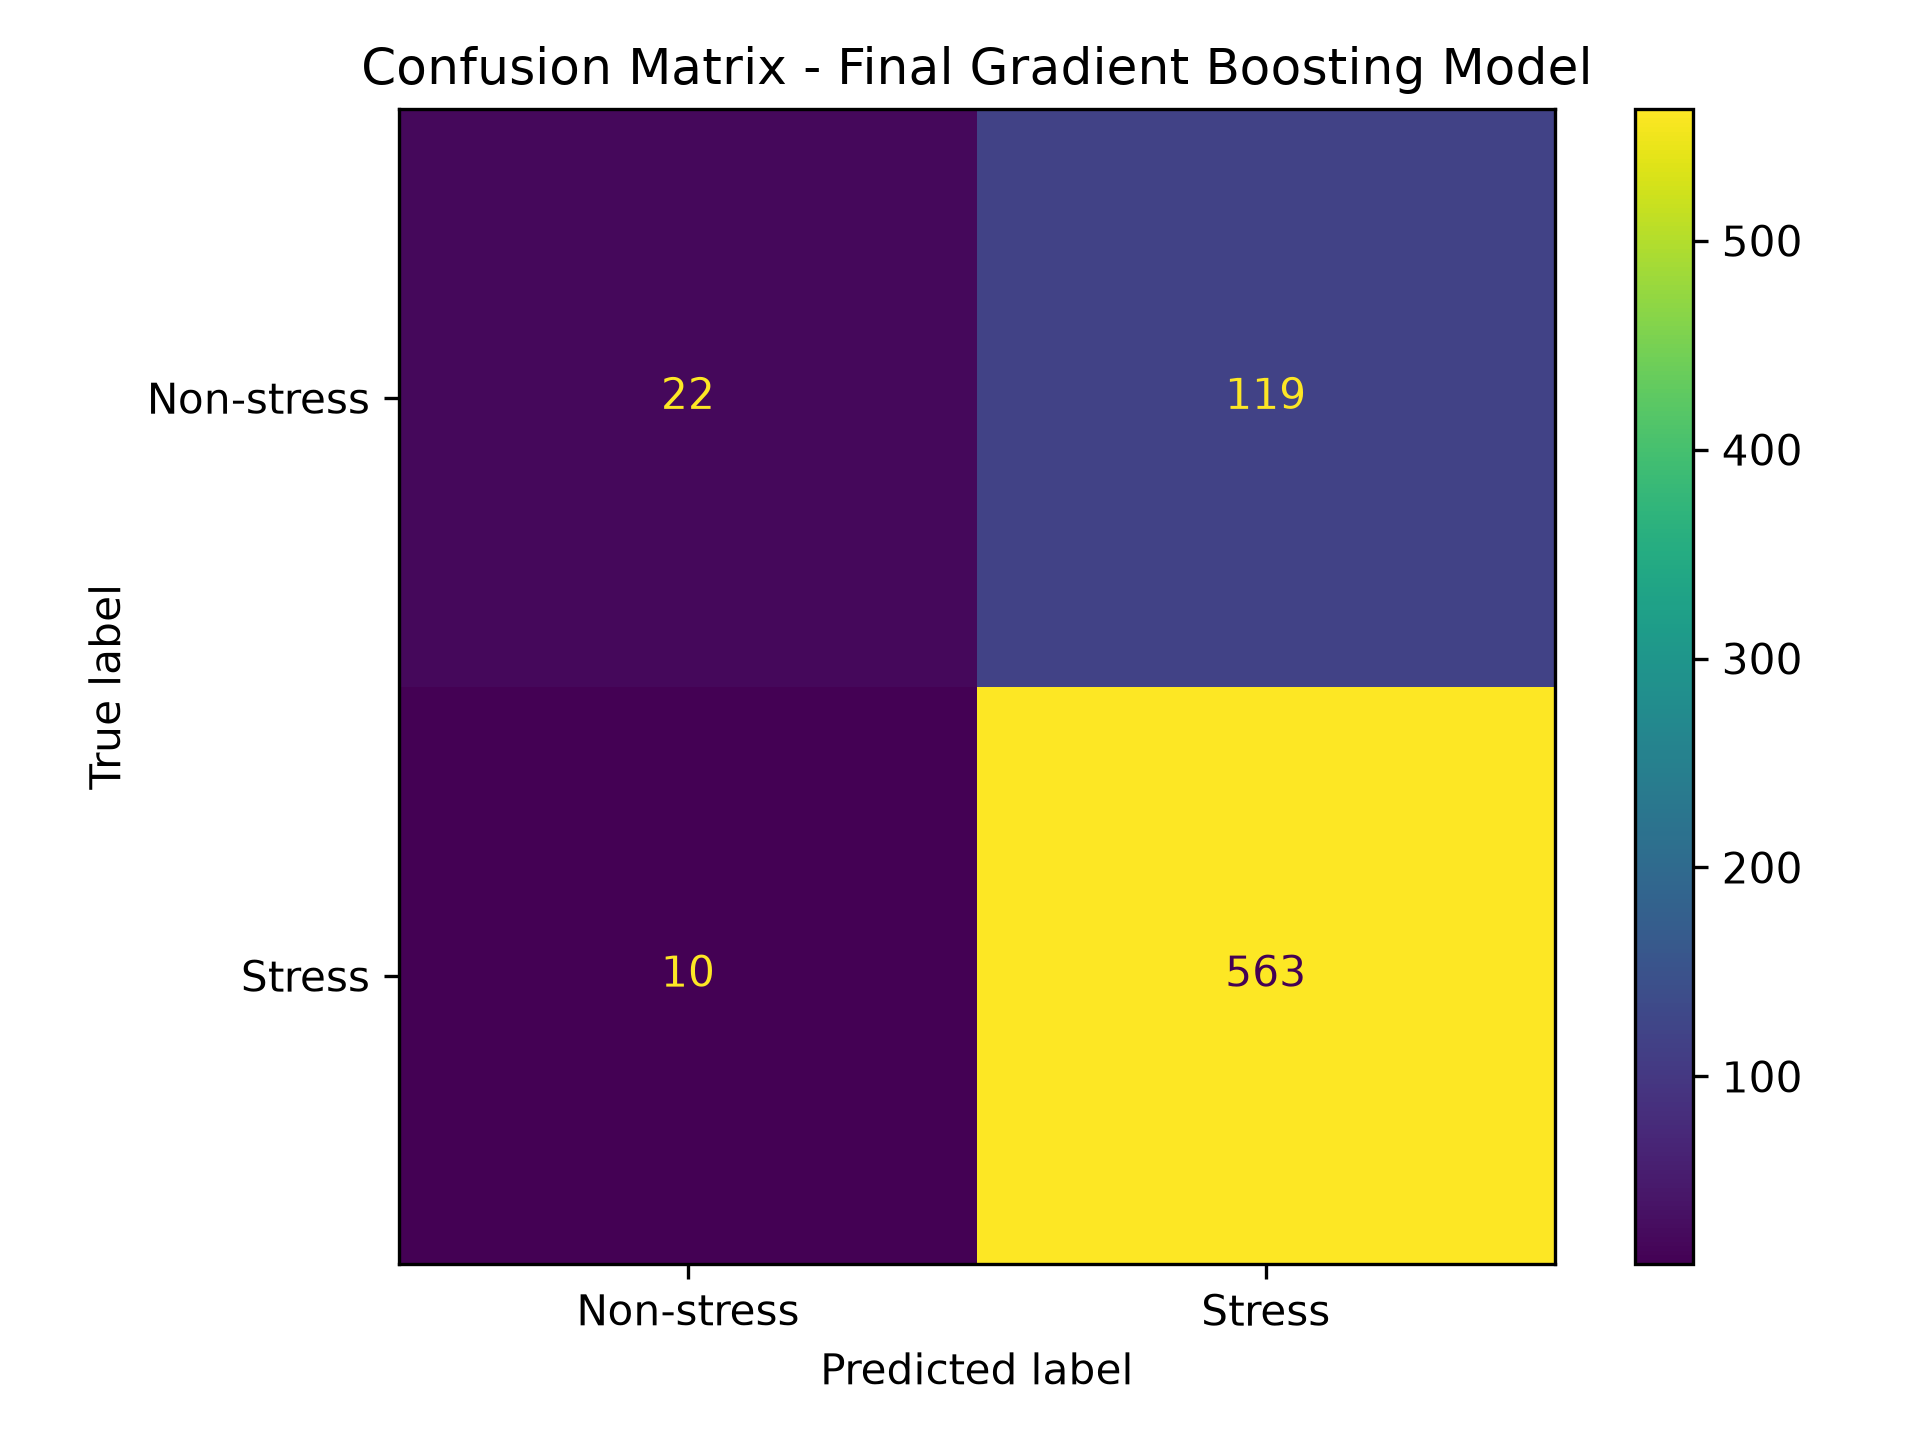
\includegraphics[width=0.75\textwidth]{../outputs/plots/confusion_matrix_final_model.png}
		\caption{Confusion matrix of the final Gradient Boosting model.}
		\label{fig:confusion_matrix}
	\end{figure}
	
	\subsection{Feature Importance}
	
	\begin{figure}[H]
		\centering
		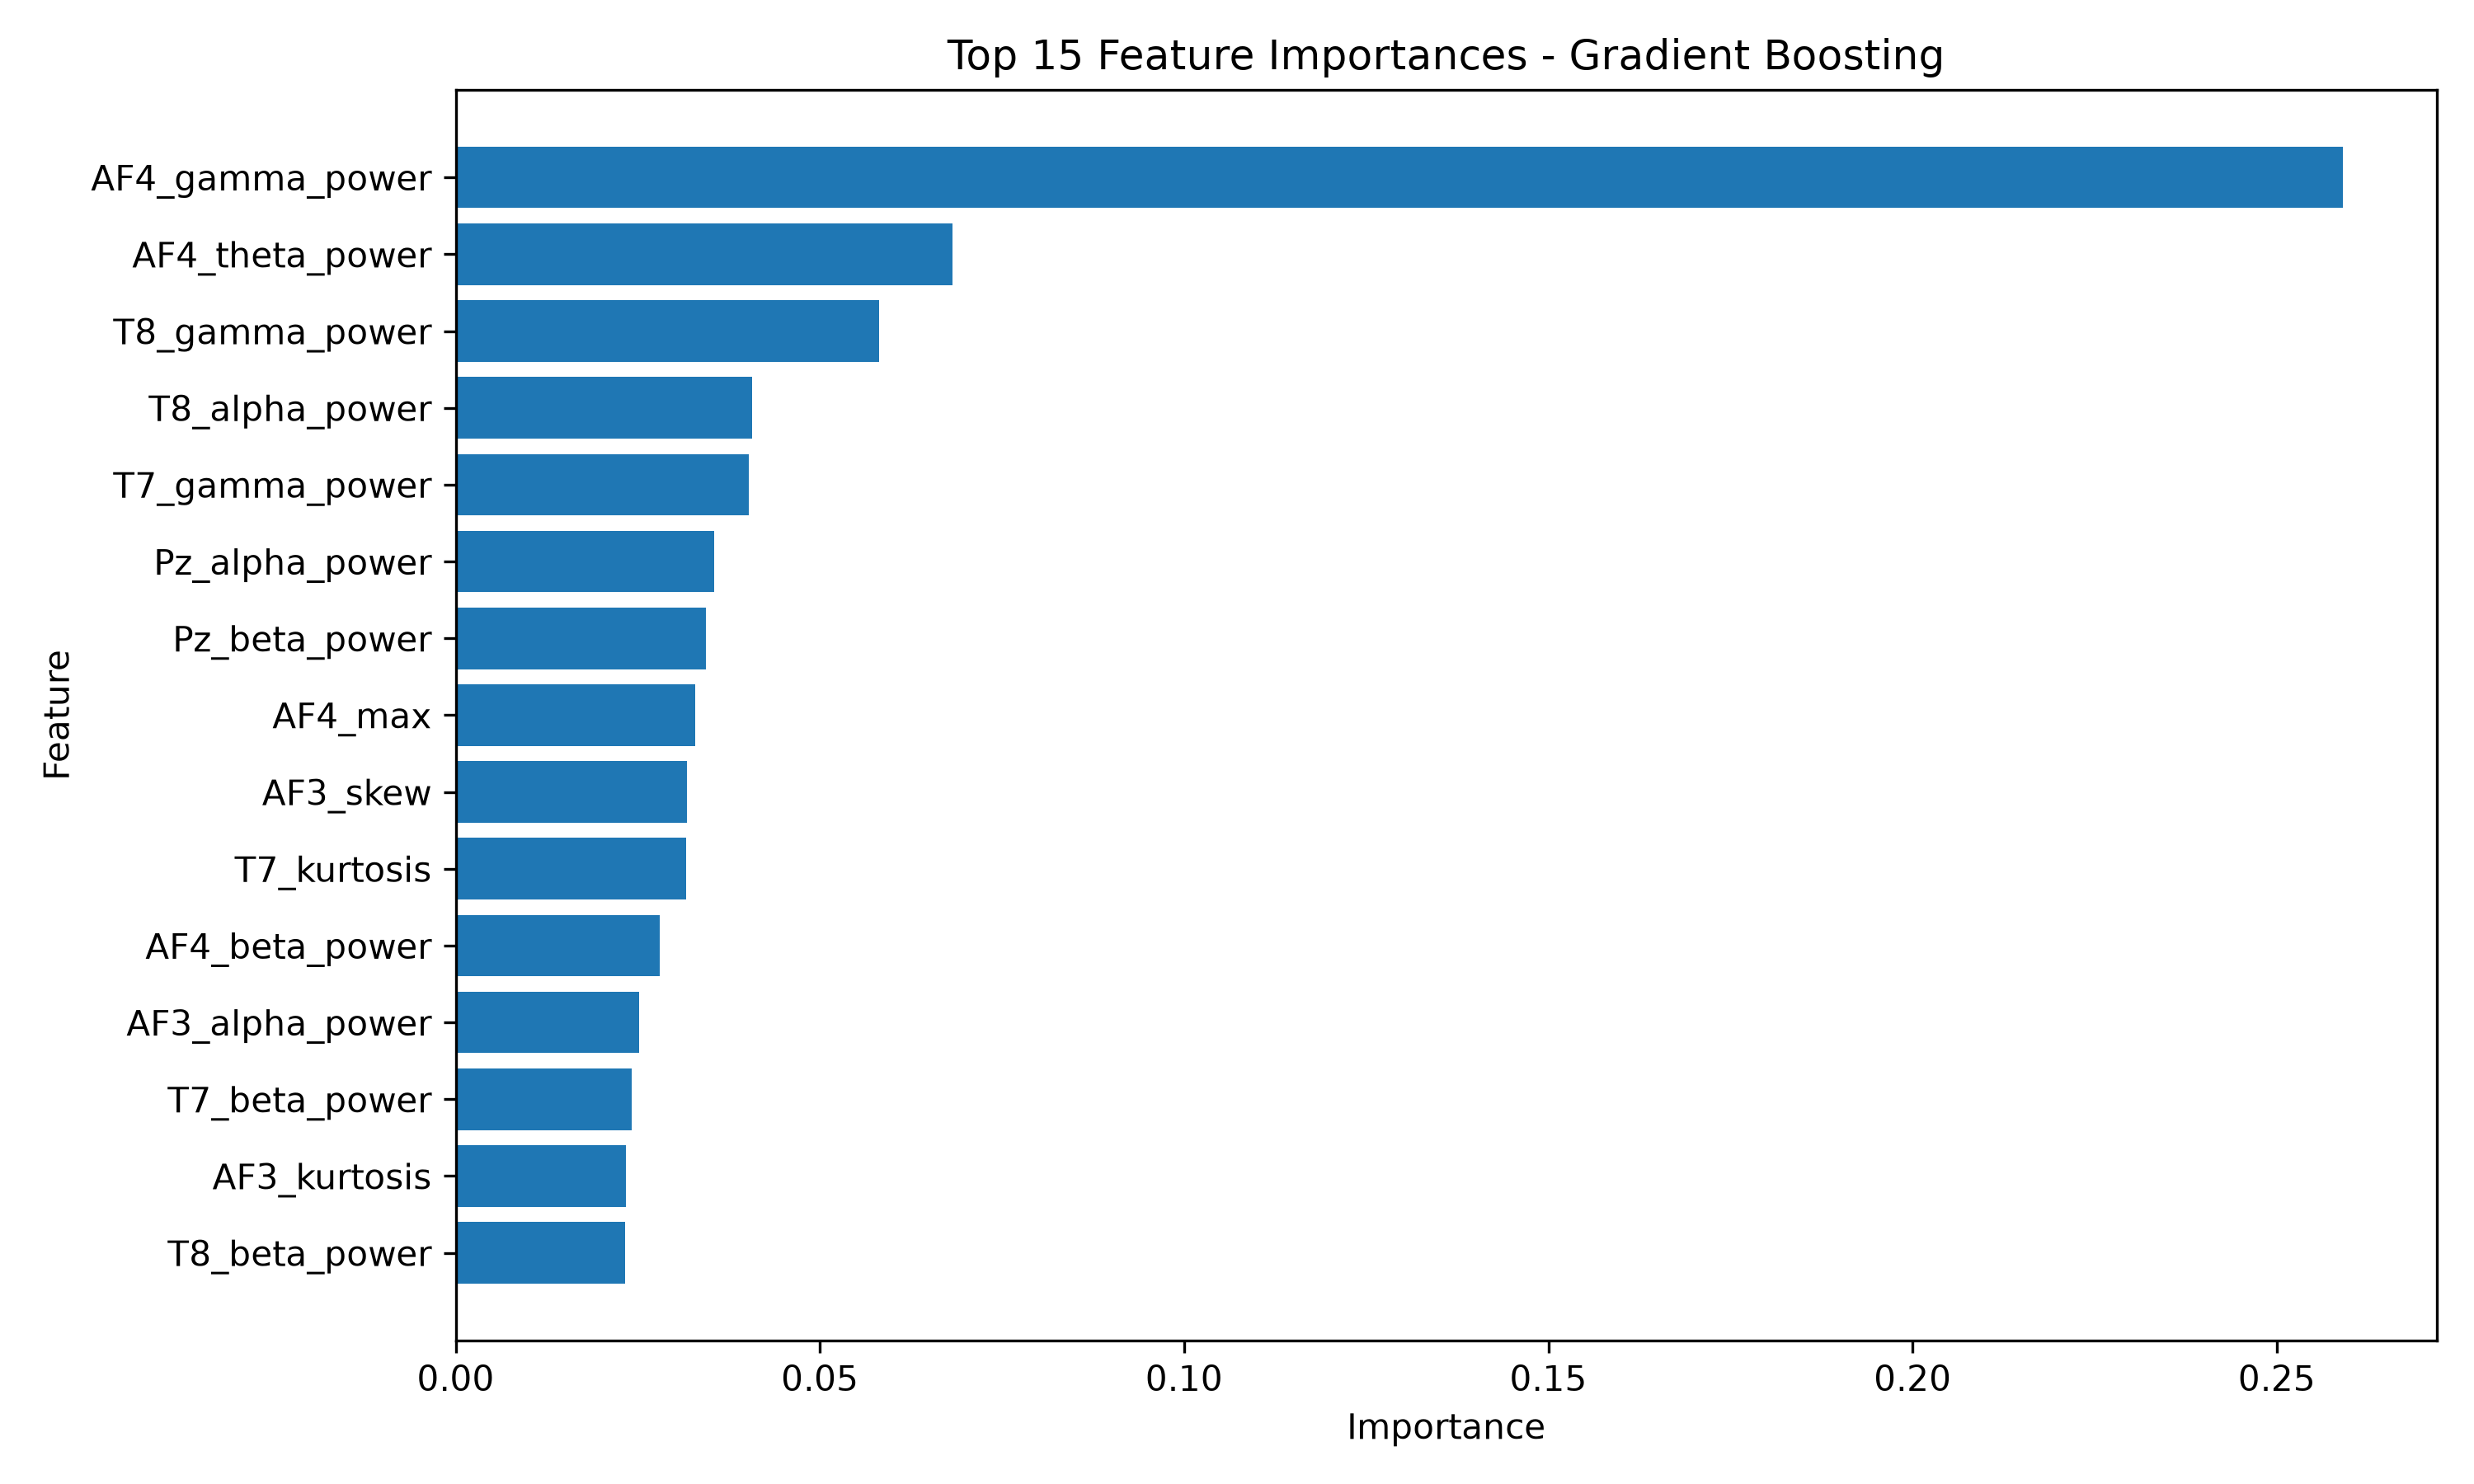
\includegraphics[width=0.9\textwidth]{../outputs/plots/feature_importance_final_model.png}
		\caption{Top 15 feature importances of the final Gradient Boosting model.}
		\label{fig:feature_importance}
	\end{figure}
	
	% =====================================================
	% 5. DISCUSSION
	% =====================================================
	\section{Discussion}
	
	% We will fill this section later.
	
	% =====================================================
	% 6. CONCLUSION
	% =====================================================
	\section{Conclusion}
	
	% We will fill this section later.
	
	% =====================================================
	% BIBLIOGRAPHY
	% =====================================================
	\newpage
	\begin{thebibliography}{9}
		
		\bibitem{dataset}
		Mendeley Data.
		\textit{An EEG Recordings Dataset for Mental Stress Detection}.
		Available at: \url{https://data.mendeley.com/datasets/wnshbvdxs2/1}
		
		\bibitem{mne}
		Gramfort, A. et al.
		\textit{MNE software for processing MEG and EEG data}.
		NeuroImage, 2014.
		
		\bibitem{sklearn}
		Pedregosa, F. et al.
		\textit{Scikit-learn: Machine Learning in Python}.
		Journal of Machine Learning Research, 2011.
		
	\end{thebibliography}
	
\end{document}
